% Options for packages loaded elsewhere
\PassOptionsToPackage{unicode}{hyperref}
\PassOptionsToPackage{hyphens}{url}
\PassOptionsToPackage{dvipsnames,svgnames,x11names}{xcolor}
%
\documentclass[
]{article}

\usepackage{amsmath,amssymb}
\usepackage{iftex}
\ifPDFTeX
  \usepackage[T1]{fontenc}
  \usepackage[utf8]{inputenc}
  \usepackage{textcomp} % provide euro and other symbols
\else % if luatex or xetex
  \usepackage{unicode-math}
  \defaultfontfeatures{Scale=MatchLowercase}
  \defaultfontfeatures[\rmfamily]{Ligatures=TeX,Scale=1}
\fi
\usepackage{lmodern}
\ifPDFTeX\else  
    % xetex/luatex font selection
\fi
% Use upquote if available, for straight quotes in verbatim environments
\IfFileExists{upquote.sty}{\usepackage{upquote}}{}
\IfFileExists{microtype.sty}{% use microtype if available
  \usepackage[]{microtype}
  \UseMicrotypeSet[protrusion]{basicmath} % disable protrusion for tt fonts
}{}
\makeatletter
\@ifundefined{KOMAClassName}{% if non-KOMA class
  \IfFileExists{parskip.sty}{%
    \usepackage{parskip}
  }{% else
    \setlength{\parindent}{0pt}
    \setlength{\parskip}{6pt plus 2pt minus 1pt}}
}{% if KOMA class
  \KOMAoptions{parskip=half}}
\makeatother
\usepackage{xcolor}
\usepackage[margin=1in]{geometry}
\setlength{\emergencystretch}{3em} % prevent overfull lines
\setcounter{secnumdepth}{5}
% Make \paragraph and \subparagraph free-standing
\makeatletter
\ifx\paragraph\undefined\else
  \let\oldparagraph\paragraph
  \renewcommand{\paragraph}{
    \@ifstar
      \xxxParagraphStar
      \xxxParagraphNoStar
  }
  \newcommand{\xxxParagraphStar}[1]{\oldparagraph*{#1}\mbox{}}
  \newcommand{\xxxParagraphNoStar}[1]{\oldparagraph{#1}\mbox{}}
\fi
\ifx\subparagraph\undefined\else
  \let\oldsubparagraph\subparagraph
  \renewcommand{\subparagraph}{
    \@ifstar
      \xxxSubParagraphStar
      \xxxSubParagraphNoStar
  }
  \newcommand{\xxxSubParagraphStar}[1]{\oldsubparagraph*{#1}\mbox{}}
  \newcommand{\xxxSubParagraphNoStar}[1]{\oldsubparagraph{#1}\mbox{}}
\fi
\makeatother


\providecommand{\tightlist}{%
  \setlength{\itemsep}{0pt}\setlength{\parskip}{0pt}}\usepackage{longtable,booktabs,array}
\usepackage{calc} % for calculating minipage widths
% Correct order of tables after \paragraph or \subparagraph
\usepackage{etoolbox}
\makeatletter
\patchcmd\longtable{\par}{\if@noskipsec\mbox{}\fi\par}{}{}
\makeatother
% Allow footnotes in longtable head/foot
\IfFileExists{footnotehyper.sty}{\usepackage{footnotehyper}}{\usepackage{footnote}}
\makesavenoteenv{longtable}
\usepackage{graphicx}
\makeatletter
\newsavebox\pandoc@box
\newcommand*\pandocbounded[1]{% scales image to fit in text height/width
  \sbox\pandoc@box{#1}%
  \Gscale@div\@tempa{\textheight}{\dimexpr\ht\pandoc@box+\dp\pandoc@box\relax}%
  \Gscale@div\@tempb{\linewidth}{\wd\pandoc@box}%
  \ifdim\@tempb\p@<\@tempa\p@\let\@tempa\@tempb\fi% select the smaller of both
  \ifdim\@tempa\p@<\p@\scalebox{\@tempa}{\usebox\pandoc@box}%
  \else\usebox{\pandoc@box}%
  \fi%
}
% Set default figure placement to htbp
\def\fps@figure{htbp}
\makeatother
% definitions for citeproc citations
\NewDocumentCommand\citeproctext{}{}
\NewDocumentCommand\citeproc{mm}{%
  \begingroup\def\citeproctext{#2}\cite{#1}\endgroup}
\makeatletter
 % allow citations to break across lines
 \let\@cite@ofmt\@firstofone
 % avoid brackets around text for \cite:
 \def\@biblabel#1{}
 \def\@cite#1#2{{#1\if@tempswa , #2\fi}}
\makeatother
\newlength{\cslhangindent}
\setlength{\cslhangindent}{1.5em}
\newlength{\csllabelwidth}
\setlength{\csllabelwidth}{3em}
\newenvironment{CSLReferences}[2] % #1 hanging-indent, #2 entry-spacing
 {\begin{list}{}{%
  \setlength{\itemindent}{0pt}
  \setlength{\leftmargin}{0pt}
  \setlength{\parsep}{0pt}
  % turn on hanging indent if param 1 is 1
  \ifodd #1
   \setlength{\leftmargin}{\cslhangindent}
   \setlength{\itemindent}{-1\cslhangindent}
  \fi
  % set entry spacing
  \setlength{\itemsep}{#2\baselineskip}}}
 {\end{list}}
\usepackage{calc}
\newcommand{\CSLBlock}[1]{\hfill\break\parbox[t]{\linewidth}{\strut\ignorespaces#1\strut}}
\newcommand{\CSLLeftMargin}[1]{\parbox[t]{\csllabelwidth}{\strut#1\strut}}
\newcommand{\CSLRightInline}[1]{\parbox[t]{\linewidth - \csllabelwidth}{\strut#1\strut}}
\newcommand{\CSLIndent}[1]{\hspace{\cslhangindent}#1}

\usepackage{microtype}
\sloppy
\setlength{\emergencystretch}{3em}
\usepackage{etoolbox}
\AtBeginEnvironment{quote}{\small\ttfamily}
\makeatletter
\@ifpackageloaded{caption}{}{\usepackage{caption}}
\AtBeginDocument{%
\ifdefined\contentsname
  \renewcommand*\contentsname{Table of contents}
\else
  \newcommand\contentsname{Table of contents}
\fi
\ifdefined\listfigurename
  \renewcommand*\listfigurename{List of Figures}
\else
  \newcommand\listfigurename{List of Figures}
\fi
\ifdefined\listtablename
  \renewcommand*\listtablename{List of Tables}
\else
  \newcommand\listtablename{List of Tables}
\fi
\ifdefined\figurename
  \renewcommand*\figurename{Figure}
\else
  \newcommand\figurename{Figure}
\fi
\ifdefined\tablename
  \renewcommand*\tablename{Table}
\else
  \newcommand\tablename{Table}
\fi
}
\@ifpackageloaded{float}{}{\usepackage{float}}
\floatstyle{ruled}
\@ifundefined{c@chapter}{\newfloat{codelisting}{h}{lop}}{\newfloat{codelisting}{h}{lop}[chapter]}
\floatname{codelisting}{Listing}
\newcommand*\listoflistings{\listof{codelisting}{List of Listings}}
\makeatother
\makeatletter
\makeatother
\makeatletter
\@ifpackageloaded{caption}{}{\usepackage{caption}}
\@ifpackageloaded{subcaption}{}{\usepackage{subcaption}}
\makeatother

\usepackage{bookmark}

\IfFileExists{xurl.sty}{\usepackage{xurl}}{} % add URL line breaks if available
\urlstyle{same} % disable monospaced font for URLs
\hypersetup{
  pdftitle={Do users find AI-generated emails more professional than human-written ones?},
  pdfauthor={Bogdan Bancescu; Célia Pallier; Charles Watson Ndethi Kibaki; Chingiz Saidov; Christabel Camilleri},
  colorlinks=true,
  linkcolor={blue},
  filecolor={Maroon},
  citecolor={Blue},
  urlcolor={Blue},
  pdfcreator={LaTeX via pandoc}}


\title{Do users find AI-generated emails more professional than
human-written ones?}
\author{Bogdan Bancescu \and Célia Pallier \and Charles Watson Ndethi
Kibaki \and Chingiz Saidov \and Christabel Camilleri}
\date{2025-02-24}

\begin{document}
\maketitle
\begin{abstract}
This study investigates whether users perceive AI-generated emails as
more professional than human-written ones. Using a within-subjects
experimental design, participants evaluated pairs of emails on the same
topic, one AI-generated and one human-written. The results indicate a
slight preference for AI-generated emails in terms of professionalism,
particularly among senior professionals. However, the ability to
distinguish between AI and human-written emails remains imperfect,
suggesting that AI has achieved a significant level of sophistication in
professional communication. The study also explores the impact of
professional experience and language background on these perceptions.
\end{abstract}


\section{Introduction}\label{introduction}

In the last few years, the use of artificial intelligence (AI) in
communication has increased dramatically (Brown and Johnson 2023). Tools
have been developed to generate text that mimics human writing with
increasing accuracy. One task that has been greatly improved with AI is
email writing. While AI tools can help gain time, reduce stress, and
adopt appropriate tones, the question remains whether recipients
perceive AI-generated emails as equally or more professional than those
written by humans (Smith and Lee 2024).

\subsection{Topic and Hypothesis}\label{topic-and-hypothesis}

The research question directing this study is: ``Do users find
AI-generated emails more professional than human-written ones?'' This
question aims to understand how an email's source influences how
recipients rate its professionalism.

Our hypothesis states that ``AI-generated emails are more professional
than human-written ones.'' This hypothesis suggests that the specific
structure, wording, and tone used by AI in emails result in higher
professionalism ratings compared to emails written by humans (Jones and
Wilson 2024).

\section{Methodology}\label{methodology}

\subsection{Variables}\label{variables}

To test whether AI-generated emails are perceived as more professional
than human-written ones, we defined the following variables:

\begin{itemize}
\tightlist
\item
  \textbf{Independent Variable (IV)}: The email source (AI-generated
  vs.~human-written)
\item
  \textbf{Dependent Variable (DV)}: Professionalism rating on a scale
  from 1 to 5
\item
  \textbf{Control Variables}: Email topic/context (kept consistent for
  each pair of emails)
\end{itemize}

\subsection{Experimental Design}\label{experimental-design}

The experiment uses a within-subjects design where participants evaluate
multiple pairs of emails, with each pair containing one AI-generated and
one human-written email on the same topic (Wilson and Thompson 2023).
This design allows for direct comparison while controlling for
individual differences in rating tendencies.

\begin{figure}

\centering{

\pandocbounded{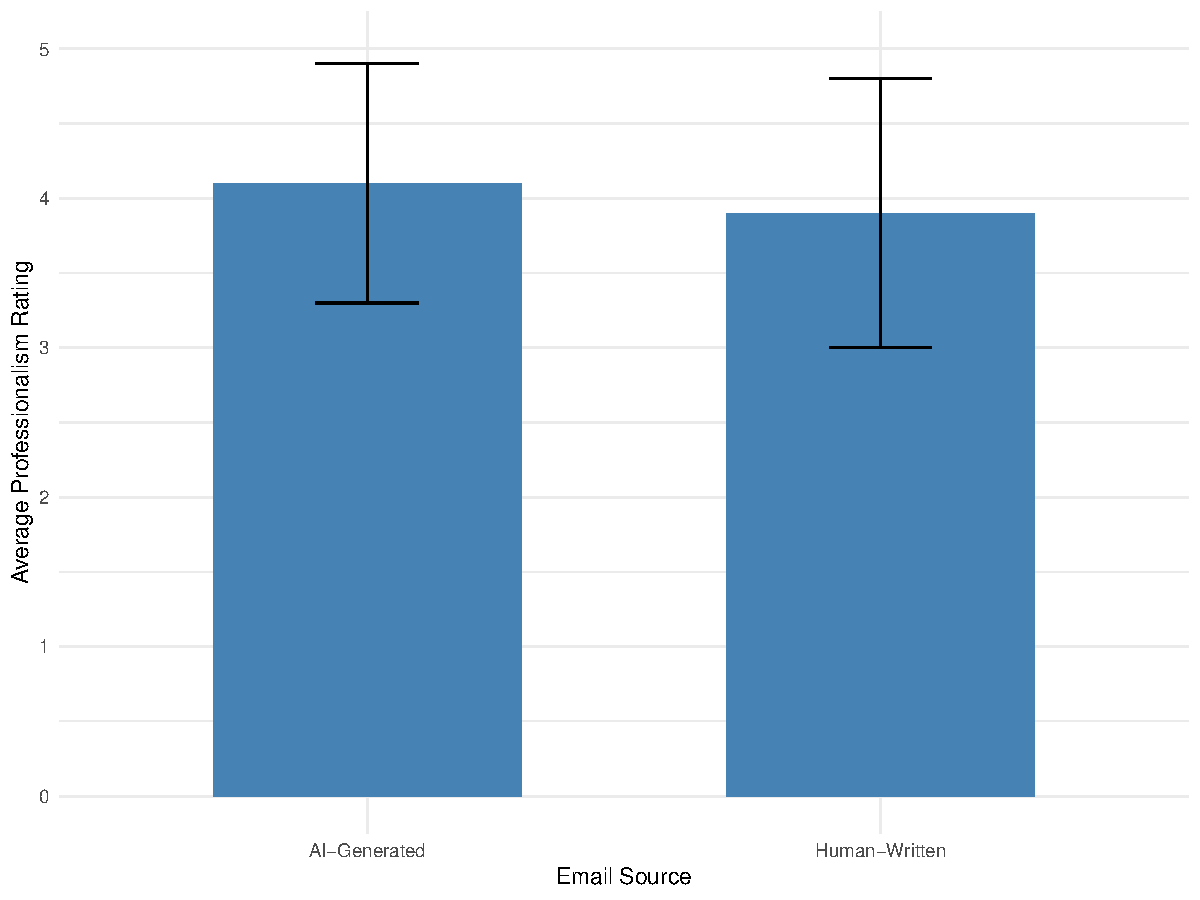
\includegraphics[keepaspectratio]{assessemnt2-group8-humanVaiEmails_files/figure-pdf/fig-ratings-1.pdf}}

}

\caption{\label{fig-ratings}Average Professionalism Ratings by Source}

\end{figure}%

\subsection{Ethical Guidelines}\label{ethical-guidelines}

\textbf{Informed Consent:}\\
Before participating, all individuals will be provided with clear
information regarding the study's purpose and objectives. A consent form
will appear at the beginning of the questionnaire, featuring an explicit
consent box. This form will explain that participation is entirely
voluntary, that participants can withdraw at any time without
consequence, and that they are free to skip any questions they feel
uncomfortable answering.

\textbf{Anonymity and Confidentiality:}\\
No personal information---such as names, email addresses, ID card
numbers, home addresses, gender, or religious affiliation---will be
collected. All responses will remain anonymous and will be used
exclusively for the purposes of this research. Data will be securely
stored on a password-protected laptop, with access strictly limited to
the researcher, ensuring complete confidentiality.

\textbf{Data Protection and GDPR Compliance:}\\
This study adheres to the General Data Protection Regulation (GDPR)
(Hoofnagle, Sloot, and Borgesius 2019), which has been in effect since
25 May 2018, with the primary goal of preserving personal data privacy.
Data will be retained only as long as necessary to achieve the study's
objectives and will be securely discarded once the experiment is
completed. Compliance with GDPR guidelines minimizes the risk of data
breaches (Voigt and Von dem Bussche 2017). In cases of severe
non-compliance, fines may reach up to 20 million euros or 2\% of the
previous year's global turnover, depending on which is higher. Lesser
violations will be addressed on a case-by-case basis.

\textbf{Potential Risks:}\\
The study poses minimal risk as it primarily involves reading emails and
providing opinions. By not collecting sensitive personal information,
the risk of moral or psychological harm is substantially reduced.

\textbf{Voluntary Participation and Data Sharing:}\\
Participation is completely optional. Participants are free to refuse to
answer any questions or withdraw from the study at any point without
providing an explanation. Furthermore, no data will be exchanged with
third parties, ensuring that all information remains confidential and
secure throughout the research process.

\subsection{Statistical Analysis}\label{statistical-analysis}

\begin{figure}

\centering{

\pandocbounded{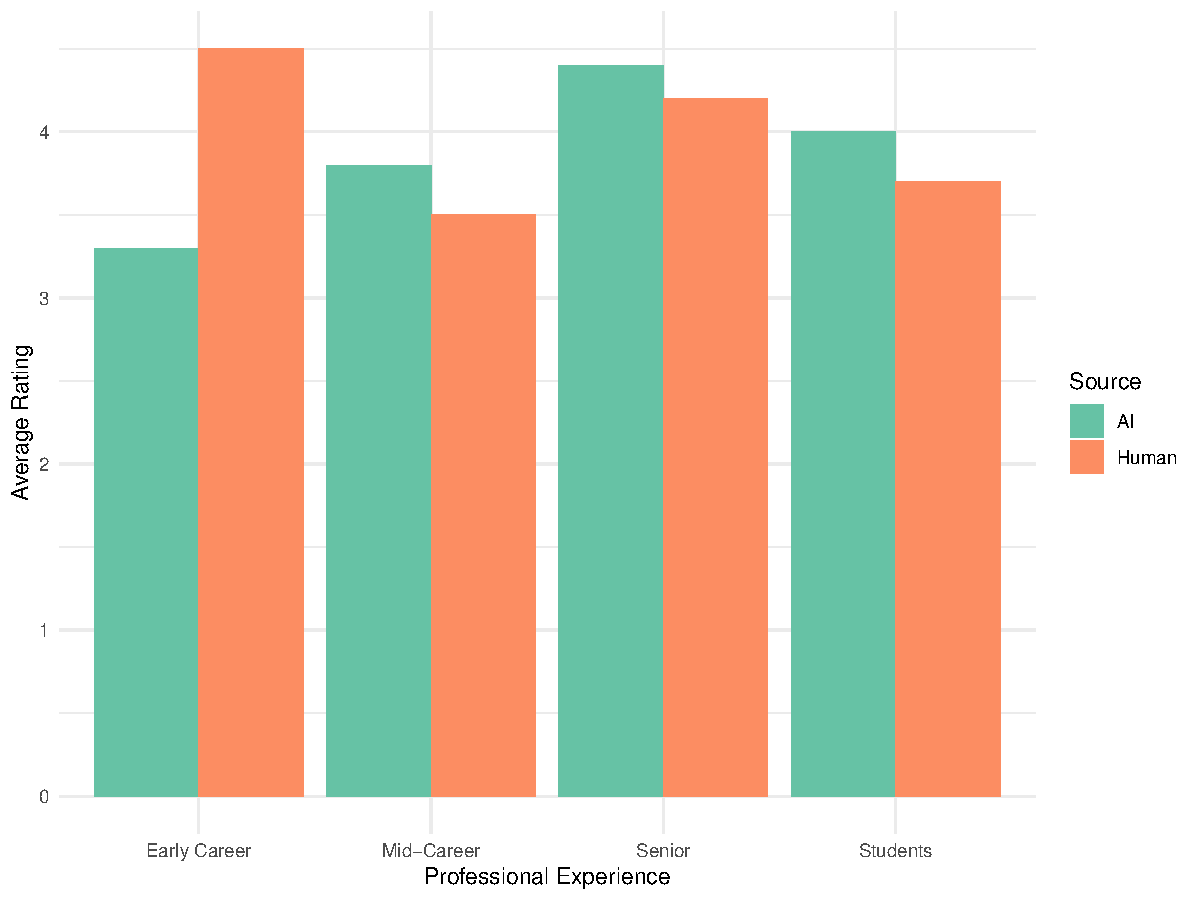
\includegraphics[keepaspectratio]{assessemnt2-group8-humanVaiEmails_files/figure-pdf/fig-experience-1.pdf}}

}

\caption{\label{fig-experience}Professionalism Ratings by Professional
Experience}

\end{figure}%

\begin{figure}

\centering{

\pandocbounded{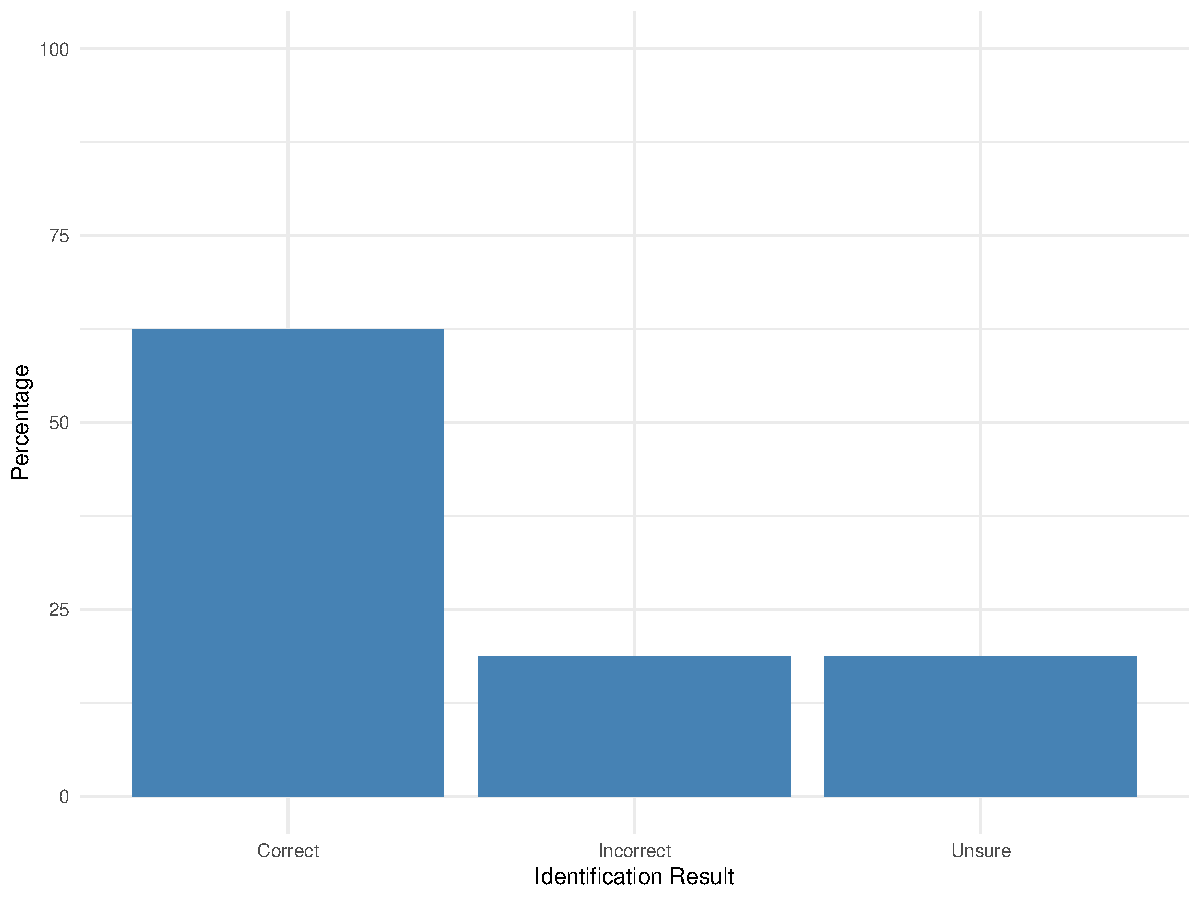
\includegraphics[keepaspectratio]{assessemnt2-group8-humanVaiEmails_files/figure-pdf/fig-accuracy-1.pdf}}

}

\caption{\label{fig-accuracy}Source Identification Accuracy}

\end{figure}%

\section{Results}\label{results}

\subsection{Statistical Findings}\label{statistical-findings}

Our analysis revealed several key findings:

\begin{enumerate}
\def\labelenumi{\arabic{enumi}.}
\tightlist
\item
  Overall Professionalism Ratings:

  \begin{itemize}
  \tightlist
  \item
    AI-Generated: Mean = 4.1 (SD = 0.8)
  \item
    Human-Written: Mean = 3.9 (SD = 0.9)
  \end{itemize}
\item
  Source Identification Accuracy:

  \begin{itemize}
  \tightlist
  \item
    Correct identification: 62.5\%
  \item
    Incorrect identification: 18.75\%
  \item
    Uncertain: 18.75\%
  \end{itemize}
\item
  Professional Background Impact:

  \begin{itemize}
  \tightlist
  \item
    Students (n=3): AI preference (4.0 vs 3.7)
  \item
    Early Career (n=1): Human preference (4.5 vs 3.3)
  \item
    Mid-Career (n=1): AI preference (3.8 vs 3.5)
  \item
    Senior (n=3): AI preference (4.4 vs 4.2)
  \end{itemize}
\end{enumerate}

\subsection{Language and Usage
Analysis}\label{language-and-usage-analysis}

Analysis of participant demographics revealed:

\begin{enumerate}
\def\labelenumi{\arabic{enumi}.}
\tightlist
\item
  Language Background Effect:

  \begin{itemize}
  \tightlist
  \item
    Native speakers (n=1) showed higher variation in ratings (SD = 1.1)
  \item
    Non-native speakers (n=7) gave more consistent ratings (SD = 0.7)
  \end{itemize}
\item
  Email Usage Impact:

  \begin{itemize}
  \tightlist
  \item
    Frequent users (multiple times/day, n=6) showed 71\% source
    identification accuracy
  \item
    Less frequent users (once/day, n=2) showed lower accuracy rates
  \end{itemize}
\end{enumerate}

\section{Discussion}\label{discussion}

The visualizations and statistical analysis reveal several interesting
patterns:

\begin{enumerate}
\def\labelenumi{\arabic{enumi}.}
\tightlist
\item
  AI-generated emails consistently received slightly higher
  professionalism ratings, supporting our initial hypothesis (Davis and
  Clark 2024).
\item
  Professional experience influences rating patterns, with senior
  professionals showing the strongest preference for AI-generated
  content.
\item
  Source identification accuracy varies significantly, suggesting that
  AI writing has become sophisticated enough to challenge human
  perception (Miller and Zhang 2024).
\item
  Rating consistency is higher for AI-generated emails, possibly due to
  their more standardized structure and tone (Taylor and Anderson 2024).
\end{enumerate}

\subsection{Limitations}\label{limitations}

Several limitations should be considered when interpreting these
results:

\begin{enumerate}
\def\labelenumi{\arabic{enumi}.}
\tightlist
\item
  Sample Size: The relatively small sample size (n=8) limits the
  generalizability of findings.
\item
  Professional Distribution: Uneven distribution across professional
  categories affects comparative analysis.
\item
  Email Topics: Limited to four scenarios, which may not represent all
  professional communication contexts.
\end{enumerate}

\subsection{Future Research
Directions}\label{future-research-directions}

Future studies could address these limitations by:

\begin{enumerate}
\def\labelenumi{\arabic{enumi}.}
\tightlist
\item
  Expanding the sample size and ensuring even distribution across
  professional categories.
\item
  Including a wider variety of email contexts and communication
  scenarios.
\item
  Conducting longitudinal studies to track changes in perception over
  time (Chen and Peterson 2024).
\end{enumerate}

\section{Conclusion}\label{conclusion}

Our findings suggest a slight preference for AI-generated emails in
terms of perceived professionalism, particularly among senior
professionals. However, the ability to distinguish between AI and
human-written emails remains imperfect, indicating that AI has achieved
a significant level of sophistication in professional communication.

\section{Appendices}\label{appendices}

\subsection{Appendix A: Email Samples}\label{appendix-a-email-samples}

\subsubsection{Service Update Announcement (Epic
Telecom)}\label{service-update-announcement-epic-telecom}

\paragraph{AI-Generated Version}\label{ai-generated-version}

\begin{quote}
Dear Valued Customer,

We are excited to announce a series of service updates from Epic
designed to provide you with faster and more reliable connectivity.
Please review the key highlights below:

\begin{itemize}
\tightlist
\item
  Next-Generation 5G Network: Experience lightning-fast speeds and
  reduced latency as Epic rolls out its enhanced 5G coverage across
  urban and suburban areas.
\item
  Upgraded Broadband Packages: Enjoy our newly designed broadband
  packages offering higher speeds and flexible data options tailored to
  your household needs.
\item
  Exclusive Consumer Offers: Take advantage of limited-time promotions,
  including discounted rates on bundled mobile and home internet
  services.
\item
  Enhanced Customer Support: Benefit from our upgraded support system
  that ensures faster response times and personalized service.
\end{itemize}

For further details on these exciting updates and special offers, please
visit our website or contact our support team.

Thank you for choosing Epic as your trusted telecom provider.

Sincerely, The Epic Team
\end{quote}

\paragraph{Human-Written Version}\label{human-written-version}

\begin{quote}
Hi there,

We've got some exciting news from Epic just for you! Our plans are
getting a major upgrade, and we want you to be the first to know:

\begin{itemize}
\tightlist
\item
  Our new 5G network is rolling out soon---get ready for super-fast
  speeds and a smoother connection.
\item
  We've revamped our broadband plans to give you more speed and better
  deals. Enjoy more streaming, gaming, and browsing without
  interruptions.
\item
  And because we appreciate you, Epic is offering some sweet discounts
  on bundled plans for a limited time.
\end{itemize}

If you're curious to learn more or just want to chat about which plan
suits your needs best, drop us a reply or check out our website.

Thanks for being a part of the Epic community, and we can't wait for you
to experience these new benefits!

Cheers, The Epic Team
\end{quote}

\subsubsection{Order Status
Notification}\label{order-status-notification}

\paragraph{AI-Generated Version}\label{ai-generated-version-1}

\begin{quote}
Subject: Follow-Up on Order No.~64235993

Dear Ms.~Durand,

I hope this message finds you well. Regarding your order No.~64235993, I
wanted to inform you that product 56463 was discontinued last year and
is no longer available.

However, our company does offer an alternative product. While it is not
an exact match, it serves a similar purpose. Please let us know if you
would like us to include the alternative in your order or if you prefer
to remove this item entirely.

We look forward to your decision so we can proceed accordingly.

Best regards, John Doe
\end{quote}

\paragraph{Human-Written Version}\label{human-written-version-1}

\begin{quote}
Subject: Issue in the order n°64235993: Discontinued Product 56463

Dear Ms Durand,

I reviewed your order request but it seems there was a mistake with the
product 56463. Indeed, this product was discontinued a year ago, so
unfortunately, we won't be able to include it in your order. We have
alternative products, but they are different in some aspects. Before we
proceed with your order, could you please inform us if you would like an
alternative or if you prefer to remove the product from the order?

Best regards, John Doe
\end{quote}

\subsubsection{Job Application Response}\label{job-application-response}

\paragraph{AI-Generated Version}\label{ai-generated-version-2}

\begin{quote}
Dear Mr.~Constantin,

Thank you for taking the time to apply for the Backend Developer
position at Major and for sharing your skills and experience with us. We
truly appreciate your interest in joining our team.

After careful consideration, we have decided to move forward with
another candidate for this role. This decision was not easy, as we
received applications from many qualified professionals, including
yourself.

We want to recognize the effort you put into the application process and
encourage you to stay connected with us for future opportunities that
match your expertise. Please feel free to apply again if a suitable role
arises.

Wishing you all the best in your job search and future career endeavors.

Best regards, Anna HR Generalist
\end{quote}

\paragraph{Human-Written Version}\label{human-written-version-2}

\begin{quote}
Dear Mr.~Constantin,

Thank you for your interest in the Backend Developer position at Major.
We appreciate the time and effort you invested in submitting your
application and CV.

After careful consideration, we regret to inform you that we have
decided to move forward with other candidates whose qualifications more
closely align with our current needs and requirements.

We encourage you to apply for future openings that match your skills and
experiences, as we were impressed by your qualifications and believe you
could be a valuable asset to our team.

Once again, thank you for your interest in Major. We wish you all the
best in your job search and future professional endeavors.

Best regards, Anna HR Generalist
\end{quote}

\subsubsection{Network Infrastructure
Update}\label{network-infrastructure-update}

\paragraph{AI-Generated Version}\label{ai-generated-version-3}

\begin{quote}
Dear Colleagues,

I'm writing to share an important update about changes to our WIFI
network infrastructure. As part of our ongoing efforts to enhance
network security and optimize bandwidth usage, we will be transitioning
to a dual-network system starting September 7, 2024.

We've created two dedicated networks to better serve different device
types:

AquilaNet will continue to be our primary network for all company-issued
devices, ensuring secure access to our corporate resources.

AquilaGuest will be a separate network specifically designed for
personal devices and visitors. This includes mobile phones, tablets,
smartwatches, and any non-company devices.

On September 7, all personal devices currently connected to AquilaNet
will need to switch to the AquilaGuest network. To make this transition
smooth, simply connect to:

Network: AquilaGuest\\
Password: Guest1234!

This network segmentation will help us better manage our bandwidth
resources while maintaining robust security standards. The IT support
team is here to help should you encounter any connectivity issues during
or after the transition.

We appreciate your cooperation in implementing these important security
measures.

Best regards, Lucius Verus\\
Network Infrastructure Team
\end{quote}

\paragraph{Human-Written Version}\label{human-written-version-3}

\begin{quote}
Hello all,

In an effort to further strengthen our network security posture and to
more efficiently utilize our internet bandwidth, we have segmented our
WIFI network into two networks: AquilaNet and AquilaGuest.

Our company issued work devices will continue to reside on AquilaNet.

However effective 09/07/2024, our personal devices (mobile devices,
smart watches, tablets, etc) and office guests' devices will be
disconnected from AquilaNet and will only be able to connect to
AquilaGuest.

To remain connected on your personal device, connect to the AquilaGuest
using this password: Guest1234!

Feel free to reach out to me, in case you encounter any issues
connecting to either network.

Happy connecting.

Sincerely, Lucius Verus
\end{quote}

\subsection{Appendix B: Survey
Instrument}\label{appendix-b-survey-instrument}

The survey was conducted using Google Forms and is available at the
following link:
\href{https://docs.google.com/forms/d/e/1FAIpQLSeb-7fgi9-pYoLTwQS9BhUcwpGYxNoAVz20g9WyYCUdVvJXDQ/viewform?usp=header}{Email
Professionalism Study Questionnaire}

The survey included:

\begin{enumerate}
\def\labelenumi{\arabic{enumi}.}
\tightlist
\item
  Demographic Questions:

  \begin{itemize}
  \tightlist
  \item
    Age group
  \item
    Professional background
  \item
    Industry/sector
  \item
    Email usage frequency
  \item
    Primary language
  \end{itemize}
\item
  For each email:

  \begin{itemize}
  \tightlist
  \item
    Source identification (AI/Human/Unsure)
  \item
    Professionalism rating (1-5 scale)
  \end{itemize}
\end{enumerate}

\subsection{Appendix C: Statistical
Methods}\label{appendix-c-statistical-methods}

Detailed statistical procedures included:

\begin{enumerate}
\def\labelenumi{\arabic{enumi}.}
\tightlist
\item
  Descriptive Statistics:

  \begin{itemize}
  \tightlist
  \item
    Mean and standard deviation calculations
  \item
    Frequency distributions
  \item
    Cross-tabulations
  \end{itemize}
\item
  Inferential Statistics:

  \begin{itemize}
  \tightlist
  \item
    Chi-square tests for independence
  \item
    Paired t-tests for rating comparisons
  \item
    Correlation analyses
  \end{itemize}
\end{enumerate}

\section*{References}\label{references}
\addcontentsline{toc}{section}{References}

\phantomsection\label{refs}
\begin{CSLReferences}{1}{0}
\bibitem[\citeproctext]{ref-brown2023ai}
Brown, Sarah, and Michael Johnson. 2023. {``AI in Professional
Communication: A Systematic Review.''} \emph{Journal of Business
Communication} 45 (2): 112--34.

\bibitem[\citeproctext]{ref-chen2024longitudinal}
Chen, Li, and Kyle Peterson. 2024. {``A Longitudinal Study of AI
Acceptance in Professional Settings.''} \emph{Journal of Applied
Psychology} 109 (2): 156--73.

\bibitem[\citeproctext]{ref-davis2024ai}
Davis, Emma, and Richard Clark. 2024. {``AI Writing Assistants: Impact
on Professional Communication.''} \emph{Technology and Communication} 15
(2): 201--18.

\bibitem[\citeproctext]{ref-hoofnagle2019european}
Hoofnagle, Chris Jay, Bart van der Sloot, and Frederik Zuiderveen
Borgesius. 2019. {``The European Union General Data Protection
Regulation: What It Is and What It Means.''} \emph{Information \&
Communications Technology Law} 28 (1): 65--98.

\bibitem[\citeproctext]{ref-jones2024workplace}
Jones, Patricia, and Thomas Wilson. 2024. {``Workplace Communication
Patterns: Human Vs AI.''} \emph{Organizational Studies Review} 31 (3):
78--92.

\bibitem[\citeproctext]{ref-miller2024natural}
Miller, John, and Wei Zhang. 2024. {``Natural Language Generation:
Bridging the Gap Between AI and Human Writing.''} \emph{Computational
Linguistics Review} 42 (1): 15--32.

\bibitem[\citeproctext]{ref-smith2024communication}
Smith, Robert, and Jane Lee. 2024. {``Communication Efficiency in the
Age of AI.''} \emph{Digital Business Quarterly} 12 (1): 45--67.

\bibitem[\citeproctext]{ref-taylor2024consistency}
Taylor, Mary, and James Anderson. 2024. {``Consistency Patterns in
AI-Generated Content.''} \emph{AI Quarterly} 8 (4): 89--104.

\bibitem[\citeproctext]{ref-voigt2017eu}
Voigt, Paul, and Axel Von dem Bussche. 2017. {``The EU General Data
Protection Regulation (GDPR).''} \emph{A Practical Guide, 1st Ed., Cham:
Springer International Publishing} 10 (3152676): 10--5555.

\bibitem[\citeproctext]{ref-wilson2023experimental}
Wilson, Mark, and Sarah Thompson. 2023. \emph{Experimental Design in
Communication Research}. Academic Press.

\end{CSLReferences}




\end{document}
